\newpage
\section{Section 3.1: Conservation of Momentum}
\begin{homeworkProblem}
    3.3* A shell traveling with velocity $\mathbf{v}_0$ explodes into three pieces of equal masses. Just after the explosion, one piece has velocity $\mathbf{v}_1 = \mathbf{v}_0$ and the other two have velocities $\mathbf{v}_2$ and $\mathbf{v}_3$ that are equal in magnitude ($v_2 = v_3$) but mutually perpendicular. Find $\mathbf{v}_2$ and $\mathbf{v}_3$ and sketch the three velocities.
    \begin{callout}{Solution:}
       
        \[ m \mathbf{v}_0 = \frac{m}{3} (\mathbf{v}_0 + \mathbf{v}_2 + \mathbf{v}_3) \]
        \[ \mathbf{v}_0 = \frac{1}{2} (\mathbf{v}_2 + \mathbf{v}_3) \tag{1.1} \]

        Where:
        \[ \mathbf{v}_0 = \begin{pmatrix} v_{x0} \\ v_{y0} \end{pmatrix}, \quad
            \mathbf{v}_2 = \begin{pmatrix} v_{x2} \\ v_{y2} \end{pmatrix}, \quad
            \mathbf{v}_3 = \begin{pmatrix} v_{x3} \\ v_{y3} \end{pmatrix} \]

        For $|\textbf{v}_{2}|=|\textbf{v}_{3}|$, while being orthogonal, we can choose:
        \begin{align*}
            \mathbf{v}_2 = \begin{pmatrix} v_{x0} \\ 0 \end{pmatrix}, \quad
            \mathbf{v}_3 = \begin{pmatrix} 0 \\ v_{y0} \end{pmatrix}
        \end{align*}
        To meet equation (1.1), we need to multiply $\textbf{v}_{2}$ and $\textbf{v}_{3}$ by 2, giving us the final momentum vectors
        \[ 
            \mathbf{p}_1 = \frac{m}{3}\begin{pmatrix} v_{x0} \\ v_{y0} \end{pmatrix}, \quad
            \mathbf{p}_2 = \frac{2m}{3}\begin{pmatrix} v_{x0} \\ 0 \end{pmatrix}, \quad
            \mathbf{p}_3 = \frac{2m}{3}\begin{pmatrix} 0 \\ v_{x0} \end{pmatrix} 
        \]
        
        \vspace{1cm} \begin{center}
            \begin{tikzpicture}[scale=1.5]
                % Draw axes
                \draw[->] (-3,0) -- (3,0) node[right] {$x$};
                \draw[->] (0,-3) -- (0,3) node[above] {$y$};

                % Velocity v0
                \draw[->, thick, blue] (0,0) -- (2,2) node[midway, above left] {$\mathbf{v}_0$};

                % Velocity v1
                \draw[->, thick, red] (0,0) -- (2,2) node[pos=0.7, below right] {$\mathbf{v}_1$};

                % Velocity v2
                \draw[->, thick, green] (0,0) -- (2,0) node[midway, below] {$\mathbf{v}_2$};

                % Velocity v3
                \draw[->, thick, orange] (0,0) -- (0,2) node[midway, left] {$\mathbf{v}_3$};

                % Additional Labels
                \node at (2.5, 2.5) {Initial Shell Velocity};
                \node at (2.2, -0.5) {Velocity of Piece 2};
                \node at (-1.0, 2.2) {Velocity of Piece 3};
            \end{tikzpicture}
        \end{center}
    \end{callout}   
\end{homeworkProblem}

\begin{homeworkProblem}
    3.5** Many applications of conservation of momentum involve conservation of energy as well, and we haven't yet begun our discussion of energy. Nevertheless, you know enough about energy from your introductory physics course to handle some problems of this type. Here is one elegant example:

    An \textit{elastic collision} between two bodies is defined as a collision in which the total kinetic energy of the two bodies after the collision is the same as that before. (A familiar example is the collision between two billiard balls, which generally lose extremely little of their total kinetic energy.) Consider an elastic collision between two equal mass bodies, one of which is initially at rest. Let their velocities be $\mathbf{v}_1$ and $\mathbf{v}_2 = 0$ before the collision, and $\mathbf{v}'_1$ and $\mathbf{v}'_2$ after. Write down the vector equation representing conservation of momentum and the scalar equation which expresses that the collision is elastic. Use these to prove that the angle between $\mathbf{v}'_1$ and $\mathbf{v}'_2$ is 90°. This result was important in the history of atomic and nuclear physics: That two bodies emerged from a collision traveling on perpendicular paths was strongly suggestive that they had equal mass and had undergone an elastic collision.
    \begin{callout}{Solution:}
        
        \begin{align*} \begin{cases}
                m \textbf{v}_{1} = m \textbf{v'}_{1} + m \textbf{v'}_{2} \\ 
                \frac{m}{2}v_{1}^2 = \frac{m}{2}\left( {v'}_1 ^{2} + {v'}_{2}^{2} \right)
            \end{cases}
        \to  \quad 
        \begin{cases}
                \textbf{v}_{1} =  \textbf{v'}_{1} + \textbf{v'}_{2} \\ 
                v_{1}^2 = {v'}_1 ^{2} + {v'}_{2}^{2}
            \end{cases}
    \end{align*}

    The second equation tells us that the magnitude of velocities is conserved. 
            \begin{align*}
                |\textbf{v}_1|^{2} &= |\textbf{v'}_{1} + \textbf{v'}_{2}|^{2}  \\ 
                |\textbf{v}_1|^{2} &= |\textbf{v'}_{1}|^2 + |\textbf{v'}_{2}|^2 + 2\textbf{v'}_{1} \cdot \textbf{v'}_{2}
            \end{align*}

            For this to match the second equation, the dot product must equal zero, implying orthogonality.

    \end{callout}
\end{homeworkProblem}

\section{Section 3.2: Rockets}

\begin{homeworkProblem}
    3.8* A rocket (initial mass $m_0$) needs to use its engines to hover stationary, just above the ground.
    \begin{enumerate}[(a)]
        \item If it can afford to burn no more than a mass $\lambda m_0$ of its fuel, for how long can it hover? [Hint: Write down the condition that the thrust just balance the force of gravity. You can integrate the resulting equation by separating the variables $t$ and $m$. Take $v_{ex}$ to be constant.]
            \begin{callout}{Solution:}
                Let the motion of the rocket be constrained to one dimension. 
                    $$m \ddot{x} = 0 = -\dot{m}\dot{x} -mg$$
                Where $\dot{x}$ is said to be a constant $v_{\textrm{ex}}$. The function of mass vs. time describing this system is then:

                \begin{align*}
                    mg &= -\dot{m}v_{\textrm{ex}} \\ 
                    \frac{1}{m} \dot{m} &= -\frac{g}{v_{\textrm{ex}}} \\ 
                    \int_{m_0}^{\lambda m} \frac{1}{m} ~dm &= -\frac{g}{v_{\textrm{ex}}} \int_{0}^{t} dt \\ 
                    \ln \left| \frac{m_0 - \lambda m_0}{m_0} \right| &= -\frac{g t}{v_{\textrm{ex}}} \\ 
                    -\ln \left| 1 - \lambda \right| &= \frac{g t}{v_{\textrm{ex}}} \\ 
                    \ln \left| \frac{1}{1 - \lambda} \right| &= \frac{g t}{v_{\textrm{ex}}} \\ 
                \end{align*}

                If the rocket can only burn no more than $\lambda m_0$ of its fuel, then the time that the rocket can burn is given by
                    $$t = \frac{v_{\textrm{ex}}}{g} \ln \left| \frac{1}{1 - \lambda} \right|$$

            \end{callout}

        \item If $v_{ex} \approx 3000$ m/s and $\lambda \approx 10\%$, for how long could the rocket hover just above the earth's surface?
            \begin{callout}{Solution:}
                
                Substituting these values in gives 
                \begin{align*}
                    t &= \frac{3000}{9.8} \ln \left| \frac{1}{1 - 0.10} \right| \\
                    t &\approx 32.25321\dots ~\textrm{seconds}
                \end{align*}


            \end{callout}
    \end{enumerate}
\end{homeworkProblem}

\begin{homeworkProblem}
    3.11** 
    \begin{enumerate}[(a)]
        \item Consider a rocket traveling in a straight line subject to an external force $F^{ext}$ acting along the same line. Show that the equation of motion is
        \begin{equation}
            m\dot{v} = -\dot{m}v_{ex} + F^{ext}. \tag{3.29}
        \end{equation}
        [Review the derivation of Equation (3.6) but keep the external force term.]
        \begin{callout}{Solution:}
            
            
            Let the total momentum of the rocket plus the fuel just ejected at time \( t + dt \) be given by
            \[ P(t + dt) = (m + dm)(v + dv) - dm(v - v_{\text{ex}}) = mv + m \, dv + dm \, v_{\text{ex}}, \]
            where we have neglected the doubly small product \( dm \, dv \). Therefore, the change in total momentum is
            \begin{align*}
                dP &= P(t + dt) - P(t) \\
                &= m \, dv + dm \, v_{\text{ex}}
            \end{align*}

            Since there is a net external force \( F^{\text{ext}} \), this change of momentum would be \( F^{\text{ext}} dt \). Therefore,
            $${F}^{\text{ext}} ~dt = m~dv + dm~v_{\textrm{ext}}$$

            Dividing out by \( dt \), we can rewrite this as
            \[ m \dot{v} = {F}^{\textrm{ext}}-\dot{m}v_{\text{ex}} \]

        \end{callout}
        
        \item Specialize to the case of a rocket taking off vertically (from rest) in a gravitational field $g$, so the equation of motion becomes
        \begin{equation}
            m\dot{v} = -\dot{m}v_{ex} - mg. \tag{3.30}
        \end{equation}
        Assume that the rocket ejects mass at a constant rate, $\dot{m} = -k$ (where $k$ is a positive constant), so that $m = m_0 - kt$. Solve equation (3.30) for $v$ as a function of $t$, using separation of variables (that is, rewriting the equation so that all terms involving $v$ are on the left and all terms involving $t$ on the right).
        \begin{callout}{Solution:}
            
            Assuming $v_{\textrm{ex}}$ is constant,
            \begin{align*}
                (m_0-kt)\dot{v} &= -kv_{\textrm{ex}} - (m_0-kt)g \\ 
                \dot{v} &= \frac{-kv_{\textrm{ex}} - (m_0-kt)g}{(m_0-kt)} \\ 
                \dot{v} &= -\frac{kv_{\textrm{ex}}}{m_0-kt} - g \\ 
                \int_{v_0}^{v} dv &= -\int_{0}^{t} \left( \frac{kv_{\textrm{ex}}}{m_0-kt} + g \right) ~dt \\ 
            \end{align*}

            Let $u=m_0-kt$ and $du=m_0-k ~dt$:
            \begin{align*}
                \int_{v_0}^{v} dv &= -\frac{kv_{\textrm{ex}}}{k}\int_{m_0}^{m_0-kt} \frac{1}{u}~du - g t \\ 
                v-v_0 &= -v_{\textrm{ex}} \ln\left| \frac{m_0-kt}{m_0} \right| - g t \\
                v(t) &= v_0 - v_{\textrm{ex}} \ln\left| \frac{m_0-kt}{m_0} \right| - g t
            \end{align*}

        \end{callout}
        
        \item Using the rough data from Problem 3.7, find the space shuttle's speed two minutes into flight, assuming (what is nearly true) that it travels vertically up during this period and that $g$ doesn't change appreciably. Compare with the corresponding result if there were no gravity.
            \begin{callout}{Solution:}
                
                Problem 3.7 gives conditions:
                "The initial mass is $2 \times 10^6$ kg, the final mass (after 2 minutes) is about $1\times 10^6$ kg, the average exhaust speed $v_{\textrm{ex}}$ is about 3000 m/s, and the initial velocity is, of course, zero."
                We begin by finding a value of $k$ which gives the desired mass after $t$ seconds using the boundary condition:
                \begin{align*}
                    m &= m_0 - kt \\ 
                    1\times10^6 &= 2\times10^6 - k(120) \\ 
                    k &= \frac{25000}{3}
                \end{align*}

                \begin{align*}
                    v(t) &= \left( v_0 ~\frac{\textrm{m}}{\textrm{s}}\right) - \left( v_{\textrm{ex}} ~\frac{\textrm{m}}{\textrm{s}} \right) \ln\left| \frac{m_0-kt}{m_0} \right| - \left( g ~\frac{\textrm{m}}{\textrm{s}^2} \right) (t\textrm{~s}) \\
                    v(t) &= \left( 0 - 3000 \ln\left| \frac{2 \times 10^6-\left( \frac{25000}{3} \right)(120)}{2 \times 10^6} \right| - (9.8)(120) \right)~\frac{\textrm{m}}{\textrm{s}} \\  
                    v(t) &= -3000\ln \left(\frac{1}{2}\right)-1176 \approx 903.44154\dots ~\frac{\textrm{m}}{\textrm{s}}
                \end{align*}
            \end{callout}
        
        \item Describe what would happen to a rocket that was designed so that the first term on the right of Equation (3.30) was smaller than the initial value of the second.
            \begin{callout}{Solution:}
                
                In such a situation the rocket would fall (or not get off the ground).

            \end{callout}
    \end{enumerate}
\end{homeworkProblem}

\section{3.3: Center of Mass}

\begin{homeworkProblem}
    3.15* Find the position of the center of mass of three particles lying in the $xy$ plane at $\mathbf{r}_1 = (1, 1, 0)$, $\mathbf{r}_2 = (1, -1, 0)$, and $\mathbf{r}_3 = (0, 0, 0)$, if $m_1 = m_2$ and $m_3 = 10m_1$. Illustrate your answer with a sketch and comment.
    \begin{callout}{Solution:}
        
        As always, the center of mass is given by
        $$\textbf{R} \equiv \frac{\sum_i m_i \textbf{r}_i}{\sum_i m_i}$$
        Where 
        $$\sum m_1 \textbf{r}_{1} - m_2 \textbf{r}_{2} - \dots = 0$$

        The center of mass is then:
        \begin{align*}
            \textbf{R} &=  \frac{1}{12m_1}\left[ (m_1, m_1, 0) + (m_1, -m_1, 0) + (0,0,0) \right] \\ 
            &= \frac{1}{6m_1} (1,0,0) \\ 
            &= \frac{1}{6m_1} \boldsymbol{\hat{x}} 
        \end{align*}

        \begin{center}
            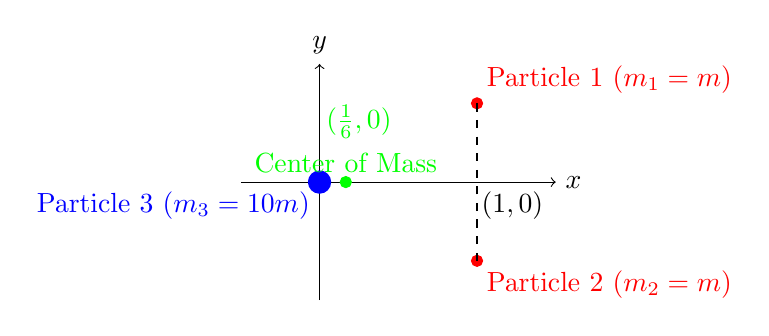
\begin{tikzpicture}
                % Draw axes
                \draw[->] (-1,0) -- (3,0) node[right] {$x$};
                \draw[->] (0,-1.5) -- (0,1.5) node[above] {$y$};

                % Draw particles
                \filldraw[red] (2,1) circle (2pt) node[above right] {Particle 1 ($m_1 = m$)};
                \filldraw[red] (2,-1) circle (2pt) node[below right] {Particle 2 ($m_2 = m$)};
                \filldraw[blue] (0,0) circle (4pt) node[below left] {Particle 3 ($m_3 = 10m$)};

                % Draw center of mass
                \filldraw[green] (2/6,0) circle (2pt) node[above] {Center of Mass};

                % Draw dashed lines to the axes
                \draw[dashed] (2,1) -- (2,0);
                \draw[dashed] (2,-1) -- (2,0);

                % Mark the coordinates
                \node[below] at (2.45,0) {$(1,0)$};
                \node[green, below] at (3/6,1.1) {$(\frac{1}{6},0)$};
            \end{tikzpicture}
        \end{center}
    \end{callout}
\end{homeworkProblem}

\begin{homeworkProblem}
    3.25* A particle of mass $m$ is moving on a frictionless horizontal table and is attached to a massless string, whose other end passes through a hole in the table, where I am holding it. Initially, the particle is moving in a circle of radius $r_0$ with angular velocity $\omega_0$, but I now pull the string down through the hole until a length $r$ remains between the hole and the particle. What is the particle's angular velocity now?
    \begin{callout}{Solution:}
        \begin{align*}
            L &= m r^2 \dot{\varphi} \\ 
            m r_0^2 \dot{\varphi}_0 &= m r^2 \dot{\varphi}_f \\ 
            r_0^2 \dot{\varphi}_0 &= r^2 \dot{\varphi}_f \\ 
            \dot{\varphi}_f &= \dot{\varphi}_0 \left( \frac{r_0}{r} \right)^2
        \end{align*}
    \end{callout}
\end{homeworkProblem}

